\section{Why the Gap Opens: A Life-Cycle Model of Careers}\label{sec:model}

The evidence leaves a puzzle. The White--Black gap in the log-wage elasticity of sons opens from 0.056 at 25--29 to
0.153 at 30--34 and 0.330 at 45--49, because the White elasticity rises with age and the Black elasticity does
not.\footnote{Hourly wages, on the model's sample of Black and White male heads aged 25--55 with a wage
(Table~\ref{tab:modelid}). The earnings gap of Section~\ref{sec:ageprofile} is zero at 25--29 because hours raise the
Black elasticity at young ages (Section~\ref{sec:contains}); the model's target is the wage, which carries the
opening.}
Sections~\ref{sec:careers}--\ref{sec:policy} locate the opening in careers after school, and point to four candidate
explanations, each a way in which race could change what parental income and schooling buy over a career:
\begin{itemize}[leftmargin=*, itemsep=0pt]
\item[H1] \textit{Access}: at equal parental income and schooling, Black sons are offered fewer jobs in which human
capital accumulates fast (Table~\ref{tab:access}).
\item[H2] \textit{The pay-off of schooling in accumulation}: a year of schooling raises the growth of human capital less
for Black sons, as the rise of the return to schooling with age within the same job suggests
(Table~\ref{tab:withincell}).
\item[H3] \textit{The entry return to schooling}: schooling is valued differently at labor-market entry, as the higher
return of Black sons at 25--29 suggests.
\item[H4] \textit{The pay-off of parental income in accumulation}: at equal schooling and job, sons of richer parents
accumulate human capital faster, and more so for White sons, as the gradient of annual wage growth at 25--34 in
parental income suggests (White 0.020$^{***}$, almost all of it with the same employer; Black $-0.001$; all
interview pairs, Table~\ref{tab:jobmoves}).
\end{itemize}
The reduced form cannot separate these: they act on the same wages over the same careers, and some of them work through
the selection of sons into jobs. This section builds one life-cycle model in which each hypothesis is one race
parameter, estimates every combination of H1--H3, with and without H4 at the two ends of that lattice, by the simulated
method of moments on the same 66 moments, and lets the data choose. Appendix~\ref{app:modelsteps} tells how the model was built, step by step.

\paragraph{Why a job side.} Models in which background acts at entry and wage profiles after entry are common
\citep[e.g.][]{lee2019intergenerational, caucutt2020early, abbott2019education} produce an IGE that changes little with
age. Models with heterogeneous ability to learn on the job \citep{huggett2011sources} do not: if learning ability is
correlated with parental income, earnings fan out with age and the log IGE rises. Such a model can produce the age
profile; it cannot produce four facts of Section~\ref{sec:careers}: about half of the White same-employer gradient is
sorting into steep jobs (Table~\ref{tab:growthladder}); the job held at 25--34 predicts half of the racial divergence
(Table~\ref{tab:earlyjob}); access to good starting jobs differs by race at equal parental income
(Table~\ref{tab:access}); and Black sons of richer parents gain less when they change employers
(Table~\ref{tab:jobmoves}). The model therefore has both sides---jobs that differ in how fast human capital accumulates,
reached through offers and search frictions, and accumulation that depends on the son's schooling and background---and
it is asked to reproduce these facts; it reproduces the first three and not the fourth (Section~\ref{sec:modelopen}). H4
is the learning-ability channel, nested and tested next to the job side.

\subsection{The model}

\paragraph{Sons.} The model follows the PSID sons from the end of school to 55, in annual periods.\footnote{The
moments are annual or biennial and the career objects are measured over five-year bands; a shorter period would add
states without adding identifying moments.} A son is described by his race $r \in \{B, W\}$, log parental income $x$
(the 13--19 mean), years of schooling $e$ and birth year, all taken from the data: each PSID son is simulated with his
own characteristics, so the schooling gradient in parental income by race is reproduced exactly and schooling is not a
choice. He enters the labor market at $18 + \max(e - 12, 0)$. He is risk neutral, discounts at $\beta$, and decides only
whether to accept job offers.\footnote{Risk neutrality is standard in job-search models with human capital
\citep[e.g.][]{bagger2014tenure}; the targets are wages, moves and displacements, not consumption. The son's hours carry
0.010 of the 0.220 (Black) and 0.012 of the 0.389 (White) elasticity of earnings at 40, so hours are not a margin. Code:
\texttt{IGE/24.IGEDecomposition.py}.}

\paragraph{Jobs, access and search frictions.} Jobs are of two types, $j \in \{G, O\}$, defined in the data and in the
simulation in the same way: $G$ is an occupation $\times$ industry cell in the top quartile of men's employment by both
CPS wage level and CPS wage growth after 35 (Table~\ref{tab:access}), $O$ any other cell. An employed son receives an
outside offer with probability $\lambda_e(a)$ a year, a son out of work with probability $\lambda_u(t)$. Every
offer---the first one at entry, offers out of work and offers on the job---is of type $G$ with probability
\begin{equation}\label{eq:modelaccess}
p(x, e, r) = \Lambda\left(\alpha_0 + \alpha_1 (x - \bar x) + \alpha_2 (e - 12) + \alpha_3\, \mathbf 1[r = B]\right),
\end{equation}
with $\Lambda$ the logistic function, and carries a match component $m' \sim N(0, \sigma_m^2)$. One access function
governs the whole career, so $\alpha_3$ is the race parameter of H1.\footnote{There is no race $\times$ parental-income
term: the racial difference in the parental-income gradient of access is $-0.022$ (s.e.\ 0.024, $p = 0.36$) once
schooling and the father's job are held fixed. The search friction on the job is common to both races: move rates at
25--34 are 0.125 (Black) and 0.130 (White). $G$ jobs carry no premium in the match component: estimated freely it is
$-0.15$ (0.17, $p = 0.38$) and fixing it at zero raises $Q$ by 2.8, within the optimiser's error; $G$ jobs differ from
$O$ jobs in accumulation. Code: \texttt{IGE/35.EarlyIndustryLatePayoff.py}, \texttt{IGE/42.SchoolingAndJobGrowth.py},
\texttt{model/hpc\_runs/ige\_full\_20261018\_200456\_j11859363}.} The on-the-job search friction declines with age,
$\lambda_e(a) = \Lambda(\ell_e + \lambda_a (a - 30)/10)$, and jobs end by displacement with probability
\begin{equation}\label{eq:modeldelta}
\delta(x, r, a, t) = \Lambda\left(\delta_{0r} + \delta_1 (x - \bar x) + \delta_a (a - 30)/10 + \phi_\delta (u_t -
\bar u)\right).
\end{equation}
The age slopes were added because a model without them could not reproduce the fall of move and displacement rates with
age.\footnote{In the PSID the displacement rate per interview pair falls from 0.173 (Black) and 0.102 (White) at 25--34
to 0.111 and 0.076 at 35--55, and the move rate from 0.131 to 0.091 (White); without age terms the model's rates rose
with age, because biennial interviews after 1997 lengthen the interval at older ages ($t$ ratios $-7.5$ and $+4.6$). The
two age slopes lower $Q$ by 111 (model A) and 112 (model D) and remove these misfits. Runs:
\texttt{model/hpc\_runs/ige\_full\_20261018\_194443\_j11859359} and \texttt{\_195922\_j11859360}.} A son displaced
in a year can find a new job in the same year, at the rate $\lambda_u(t)$ of a son out of work.\footnote{Without
same-year re-employment every displacement produced a full year without hours, so the model could not match the
displacement rates and the share of zero-hours years together, and job finding out of work went to its upper bound.
Same-year re-employment lowers $Q$ by a further 36 (models A and D) and identifies job finding out of work, estimated at
0.51. Runs: \texttt{\_200455\_j11859361}, \texttt{\_200456\_j11859362}.} The slope of displacement in parental income is
common to both races, as in the data ($-0.037^{***}$ and $-0.038^{***}$, $p < 0.01$). The national unemployment rate
$u_t$ (BLS) shifts job loss and job finding, $\lambda_u(t) = \bar\lambda_u \exp\{\phi_\lambda(u_t - \bar u)\}$, with
elasticities calibrated at $\mp 0.10$; sons hold stationary expectations about it. There is no shifter of access by
conditions at entry: the entry rate leaves average access unchanged (0.004, s.e.\ 0.008, $p = 0.62$;
Section~\ref{sec:policy}).

\paragraph{Human capital and wages.} While employed in a job of type $j$, the son's human capital level evolves as
\begin{equation}\label{eq:modelhc}
h_{a+1} = h_a + \left[\gamma_j + \gamma_1(r)\, (e - 12) + \gamma_x(r)\, (x - \bar x)\right] e^{-\rho(a - 18)} +
\eta_{a+1},
\end{equation}
and $h_{a+1} = h_a + \eta_{a+1}$ in a year out of work, with $\gamma_G - \gamma_O$ the faster accumulation on good jobs,
$\gamma_1(r)$ the pay-off of schooling in accumulation, $\gamma_x(r)$ the pay-off of parental income in accumulation,
$\rho$ the decline of accumulation with age and $\eta \sim N(0, \sigma_\eta^2)$ a permanent shock. The race parameter of
H2 is $\gamma_1(B) - \gamma_1(W)$; that of H4 is $\gamma_x(B) - \gamma_x(W)$.\footnote{The reduced form found the
parental-income gradient of same-employer growth net of schooling to be 0.008 ($p = 0.17$) in the PSID and 0.002
($p = 0.73$) in the NLSY79 (Table~\ref{tab:growthladder}, columns (4) and (9)), and a first version of the model left $\gamma_x$ out. That model
selected H2 and H3, reproduced half of the opening (a gap of 0.159 at 45--49) and fitted a White IGE too flat after 35
and a Black IGE that rose; a gradient of 0.008 a year cumulated over twenty years is about 0.16 of IGE, the missing
half, and the annual-growth regression is too noisy to detect it. Adding $\gamma_x(r)$ lowers $Q$ by 42.5 (model A at
five simulated sons per son); a race-neutral $\gamma_x$ alone lowers it by nothing ($-0.3$). Runs:
\texttt{model/hpc\_runs/ige\_full\_20261018\_213123\_j11860453}, \texttt{\_j11860454}.} Human capital does not
depreciate in a year out of work.\footnote{Estimated freely, depreciation out of work is negative ($-0.039^{***}$,
s.e.\ 0.014): wages rise across a spell without work, which the model cannot interpret; it is fixed at zero, which
raises $Q$ by 6.2. Run \texttt{\_212217\_j11860451}.} The log wage is
\begin{equation}\label{eq:modelwage}
\ln w_a = \mu_r + h_a + m_a + \varepsilon_a ,
\end{equation}
with $m_a$ the match component of the current job, lost at a move or displacement, and $\varepsilon_a \sim N(0,
\sigma_\varepsilon^2)$ a transitory shock that includes measurement error. The level $\mu_r$ ($\mu_W = 0$) is the racial
wage gap at equal human capital, the residual of \citet{neal1996role}; it is held fixed in every counterfactual. A son's
starting human capital level is $h_0 = b_0 + b_x (x - \bar x) + b_1(r) (e - 12) + \nu$, $\nu \sim N(0, \sigma_0^2)$,
so parental income enters the starting position directly as well as through schooling and access; the race parameter
of H3 is $b_1(B) - b_1(W)$.\footnote{Holding schooling fixed, the parental-income gradient of log wages at 25--29 is
0.174$^{***}$ (White) and 0.137$^{***}$ (Black), $p < 0.01$; at 25--29 the return to a year of schooling is 0.124$^{***}$
(Black) and 0.045$^{***}$ (White) in earnings, and the difference survives fixed effects for the son's early job
(0.061$^{***}$) in the PSID but not in the NLSY79 (0.008). Code: \texttt{IGE/42.SchoolingAndJobGrowth.py},
\texttt{IGE/45.WithinCellIdentification.py}.}

\paragraph{Decisions.} With $\theta = (r, x, e)$, the values of an employed son with human capital level $h$ in a job
$(m, j)$ and of a son out of work are
\begin{align}
V^E_a(h, m, j) &= e^{\mu_r + h + m + \sigma_\varepsilon^2/2} + \beta\, \mathbb{E}\Big\{\delta\, \big[\lambda_u
\max\{V^U_{a+1}(h'), V^E_{a+1}(h', m', j')\} + (1 - \lambda_u) V^U_{a+1}(h')\big] \nonumber\\
&\qquad + (1 - \delta) \big[(1 - \lambda_e) V^E_{a+1}(h', m, j) + \lambda_e \max\{V^E_{a+1}(h', m, j),
V^E_{a+1}(h', m', j')\}\big]\Big\}, \nonumber\\
V^U_a(h) &= b\, e^{\mu_r + h} + \beta\, \mathbb{E}\Big\{\lambda_u \max\{V^U_{a+1}(h'), V^E_{a+1}(h', m', j')\}
+ (1 - \lambda_u) V^U_{a+1}(h')\Big\},
\end{align}
with $h'$ from (\ref{eq:modelhc}), the value of a year out of work a share $b = 0.4$ of the potential wage, and zero
values at 55. A $G$ offer with a lower match than the current job can be accepted because it raises future
accumulation, so acceptance is forward-looking.

\subsection{What can be solved without simulation}

Three results reduce what the simulation has to do. \textit{Homogeneity}: because flows are proportional to $e^{\mu_r +
h}$ and $h' - h$ does not depend on $h$, $V^E_a(h, m, j) = e^{\mu_r + h} v^E_a(m, j)$ and $V^U_a(h) = e^{\mu_r + h}
v^U_a$ for every type and age, so decisions do not depend on $h$ or the shocks and the model is solved on the match grid
alone, exactly for each of the 4,765 PSID sons. \textit{Stayers' wage growth}: for a son who stays with his employer,
$\mathbb E[\Delta \ln w] = [\gamma_j + \gamma_1(r)(e - 12) + \gamma_x(r)(x - \bar x)] e^{-\rho(a-18)}$, because staying
is independent of $\eta$; the accumulation parameters are identified by nonlinear least squares on stayers' wage
growth, which gives starting values ($\gamma_O = 0.123^{***}$, $\gamma_G = 0.145^{***}$, $\rho = 0.090$, $\gamma_1 =
0.023^{***}$, all $p < 0.01$).\footnote{The joint estimates differ from these starting values ($\gamma_O = 0.092$,
$\gamma_G = 0.172$, $\gamma_1(W) = 0.013$; Table~\ref{tab:modelest}) because the least-squares fit pools the races,
uses only stayers' growth and ignores the selection of who is a stayer at the next interview, while the joint estimates
must also fit the six return-to-schooling bands by race and the stayers' slope in schooling (PSID 0.009, model 0.007
for White sons). The starting values are starts, not estimates.} \textit{Shock variances}: for annual stayers the lag-1 autocovariance of wage growth is
$-\sigma_\varepsilon^2$ \citep{altonji2013modeling}, which gives $\sigma_\varepsilon^2 = 0.037$. Displacement is an
exogenous hazard identified by a logit on interview pairs. The remaining parameters---the racial wage level, the
starting position, access, the search frictions and the match distribution---need the model, because the moments that
carry them are outcomes of offers and acceptance. Every parameter, including those with closed forms, is estimated
jointly; the closed forms are starting values and checks.

\subsection{Identification and estimation}

Table~\ref{tab:modelid} ties each parameter to the moments that identify it. There are 66 moments, computed with the
same code on the PSID sons and on the simulated panel: the log-wage IGE and the return to schooling by five-year band
and race (24); the mean log wage at 25--29 and the variance of log wages at 25--29, 35--39 and 45--49 by race (8); the
share whose modal job at 25--34 is a $G$ job, by race and parental-income tercile and by schooling (9); same-employer
wage growth by age and job type, by race, its slope in schooling by race, and its variance and autocovariance (10); move
and displacement rates at 25--34 and 35--55 by race, the slope of displacement in parental income, the wage growth at a
move by race and its slope in parental income, and the wage growth across a displacement (13); and the share of
zero-hours years by race (2). The simulated panel is observed as the PSID observes sons: interviews annual to 1997 and
biennial afterwards, the wage of the year before the interview, same-employer pairs one to two years apart from 1985,
and the job type of the modal job at 25--34. The four race parameters are separated by the shape of the age profiles, and the
sensitivity of each estimate to the moments \citep{andrews2017measuring} shows which moments do the work
(Appendix Table~\ref{tab:modelsens}). The racial difference in the pay-off of parental income (H4) draws 77\% of its
sensitivity from the twelve IGE moments: a higher White IGE at 30--44 makes it more negative, a higher Black IGE at
25--39 less negative. Its race-neutral counterpart $\gamma_x$ is separated from the parental-income gradient of the
starting level $b_x$ by the age profile: a higher IGE at 25--29 lowers $\gamma_x$ (the level goes to $b_x$), a higher
White IGE at 35--55 raises it. The racial differences in the entry return (H3) and in the pay-off of schooling (H2) draw
73\% and 63\% of their sensitivity from the twelve returns to schooling: H3 moves with the Black return at 25--29 ($+0.60$) and against the White return at 25--29 ($-0.41$), that
is with the racial difference in the entry return; H2 moves with the Black return at 45--55 and against the Black return
at entry, which is why the two are identified
jointly by the level and the rise of one profile. Access (H1) draws 96\% from the shares in $G$ jobs by race and
parental tercile. The counterfactual change in the gap at 45--49 when H4 is switched off draws 87\% from the IGE
moments, so it rests on the fact it explains and not on the career moments the model fits less well.

\begin{table}[!htbp]
\centering
\caption{Parameters, identifying moments and their PSID values}\label{tab:modelid}
\footnotesize
\begin{tabular}{p{3.2cm}p{6.0cm}p{5.0cm}}
\toprule
Parameter & Identifying moments & PSID values (Black / White) \\
\midrule
$\mu_B$ & mean log wage at 25--29 & 2.315 / 2.595 \\
$b_0$, $b_x$, $\sigma_0$ & mean, parental-income gradient and variance of log wages at 25--29 & IGE 0.148 / 0.205; variance 0.312 / 0.276 \\
$b_1$, $b_1(B) - b_1(W)$ (H3) & return to schooling at 25--29 & 0.067 / 0.047 \\
$\gamma_1$, $\gamma_1(B) - \gamma_1(W)$ (H2) & rise of the return to schooling with age; stayers' growth on schooling & 0.067 $\to$ 0.124 / 0.047 $\to$ 0.129; 0.003 / 0.009 \\
$\gamma_x$, $\gamma_x(B) - \gamma_x(W)$ (H4) & rise of the IGE with age, given the return to schooling by age and the $G$ shares & 0.148 $\to$ 0.140 / 0.205 $\to$ 0.470 \\
$\alpha_0$, $\alpha_1$, $\alpha_2$ & share in $G$ at 25--34 by parental tercile and schooling & terciles 0.031--0.117 / 0.066--0.180; schooling $\le$12, 13--15, 16+: 0.016, 0.050, 0.265 \\
$\alpha_3$ (H1) & share in $G$ by race at equal tercile & see the $\alpha_0$--$\alpha_2$ row \\
$\ell_e$, $\lambda_a$ & move rates without displacement by age & 25--34: 0.127 / 0.131; 35--55: 0.090 / 0.091 \\
$\bar\lambda_u$ & zero-hours years given the displacement rates & 0.110 / 0.039 \\
$\sigma_m$ & gain at a move and its parental-income slope & gain $-0.006$ / 0.052; slope $-0.016$ \\
$\delta_{0B}$, $\delta_{0W}$, $\delta_1$, $\delta_a$ & displacement rates by age and race; slope in parental income & 25--34: 0.173 / 0.102; 35--55: 0.111 / 0.076; slope $-0.017$ \\
$\gamma_O$, $\gamma_G$, $\rho$ & same-employer growth by job type at 25--34 and 35--55 & $O$: 0.055, 0.021; $G$: 0.075, 0.035 \\
$\sigma_\eta$, $\sigma_\varepsilon$ & variance of log wages by age; variance and autocovariance of stayers' growth & 0.276 $\to$ 0.504 (White); 0.121, $-0.037$ \\
\bottomrule
\end{tabular}
\par\smallskip
\begin{minipage}{\textwidth}\footnotesize \textit{Notes:} PSID sons, Black and White male heads, 25--55; 4,765 sons,
46,540 son-years. Rates per interview pair; growth annualised; IGE and returns from the band regressions with
single-age dummies; arrows give 25--29 to 45--49. Calibrated: $\beta = 0.95$, $b = 0.4$, $\phi_\lambda = -0.10$,
$\phi_\delta = 0.10$. Code: \texttt{model/build\_data.py}.\end{minipage}
\end{table}

\paragraph{Estimation.} The criterion is $Q(\vartheta) = \sum_k ((m_k(\vartheta) - \hat m_k)/\hat s_k)^2$, with $\hat s_k$
the cluster-bootstrap standard deviation of each data moment (500 draws of the 1968 families) and 20 simulated sons per
PSID son, with common random numbers across parameter values. It is minimised by CMA-ES; all parameters are estimated
jointly, with no hand tuning. Standard errors are of the sandwich form, with the bootstrap covariance of the moments in the
middle. The twelve IGE moments contribute 4.9 of the 127.6 of $Q$ at the selected model, 4\% of the criterion for
18\% of the moments, because they are fitted within their standard errors, not because they are down-weighted: their
weight is their precision.

\paragraph{The test.} H4 enters every model of the lattice, which estimates all eight combinations of H1--H3: model A
has none of them, B adds H1, F H2, G H3, C H1 and H2, H H1 and H3, E H2 and H3, and D all three. H4 is tested by
estimating A and E without it. Each model is started from the best solution of the models nested in it, so that a
richer model never starts from a worse point than a model it contains.\footnote{Re-starting the same model from a
different point moved $Q$ by 5 to 9 in earlier runs, more than the 3.84 rule; the chained starts make the lattice
coherent, and the nesting checks confirm it: across 38 pairs and ten seeds, no richer model fits worse by more than 2.3
at five simulated sons per son or 0.6 at twenty, within the seed spread. Code: \texttt{model/hpc\_ige\_chain.sh}.}
A race parameter is kept if adding it lowers $Q$ by more than 3.84 at each of ten simulation seeds; with diagonal weights
this is a rule of thumb on the scale of a one-restriction test \citep{newey1987hypothesis}, not an exact one, and the
table also reports the sandwich Wald test of the parameter.

\subsection{The verdict}

Table~\ref{tab:modelhyp} reports each hypothesis alone and given the others, and Appendix Table~\ref{tab:modellattice}
the fit of all ten models. The tests are those of the lattice; the parameter values quoted are those of the selected
model, which adds one further step, a racial difference in job finding out of work (below).

\begin{table}[!htbp]
\centering
\caption{The four hypotheses: drop in the SMM criterion when the race parameter is added}
\label{tab:modelhyp}
\resizebox{\ifdim\width>\textwidth\textwidth\else\width\fi}{!}{%
\begin{tabular}{llcccc}
\toprule
 & Models & Drop in $Q$: mean (s.d.) & Minimum & $> 3.84$ at & Estimate in the \\
 & & over ten seeds & & every seed & richer model (s.e.) \\
\midrule
\multicolumn{6}{l}{\textit{H1: access to good jobs ($\alpha_3$)}} \\
\quad alone & A $\to$ B & $3.2$ (1.0) & $1.4$ & no & $-0.2739^{*}$ (0.1530) \\
\quad given H2 & F $\to$ C & $2.5$ (0.8) & $1.4$ & no & $-0.2429$ (0.1534) \\
\quad given H3 & G $\to$ H & $2.9$ (0.9) & $1.1$ & no & $-0.2739^{*}$ (0.1508) \\
\quad given H2 and H3 & E $\to$ D & $1.4$ (0.6) & $0.5$ & no & $-0.1401$ (0.1795) \\
\multicolumn{6}{l}{\textit{H2: pay-off of schooling in accumulation ($\gamma_1(B) - \gamma_1(W)$)}} \\
\quad alone & A $\to$ F & $1.7$ (1.0) & $0.3$ & no & $-0.0020$ (0.0019) \\
\quad given H1 & B $\to$ C & $1.0$ (0.7) & $-0.2$ & no & $-0.0014$ (0.0020) \\
\quad given H3 & G $\to$ E & $9.9$ (1.3) & $8.1$ & yes & $-0.0085^{***}$ (0.0030) \\
\quad given H1 and H3 & H $\to$ D & $8.5$ (1.0) & $7.2$ & yes & $-0.0075^{**}$ (0.0030) \\
\multicolumn{6}{l}{\textit{H3: entry return to schooling ($b_1(B) - b_1(W)$)}} \\
\quad alone & A $\to$ G & $0.3$ (0.4) & $-0.6$ & no & $0.0020$ (0.0090) \\
\quad given H1 & B $\to$ H & $0.0$ (0.0) & $0.0$ & no & $0.0000$ (0.0089) \\
\quad given H2 & F $\to$ E & $8.5$ (0.8) & $7.3$ & yes & $0.0369^{***}$ (0.0138) \\
\quad given H1 and H2 & C $\to$ D & $7.5$ (0.8) & $6.6$ & yes & $0.0347^{**}$ (0.0137) \\
\multicolumn{6}{l}{\textit{H4: pay-off of parental income in accumulation ($\gamma_x(B) - \gamma_x(W)$)}} \\
\quad alone & A without H4 $\to$ A & $47.1$ (4.0) & $38.4$ & yes & $-0.0210^{***}$ (0.0056) \\
\quad given H2 and H3 & E without H4 $\to$ E & $36.1$ (3.5) & $29.1$ & yes & $-0.0198^{***}$ (0.0055) \\
\bottomrule
\end{tabular}}
\par\smallskip
\begin{minipage}{\textwidth}\footnotesize \textit{Notes:} Each row adds one race parameter to a model and reports the fall in the SMM criterion $Q$ (66 moments, diagonal weights) at the two models' estimates, computed on the same simulation draws at ten seeds (7--16), 20 simulated sons per PSID son; mean, standard deviation and minimum over the seeds. A parameter is kept if the fall exceeds 3.84 at every seed (with diagonal weights this is a rule of thumb on the scale of a one-restriction test, not an exact $\chi^2$ test). All models include the age profiles of job loss and of the on-the-job search friction, re-employment in the year of a displacement and the race-neutral pay-off of parental income in accumulation $\gamma_x(W)$; the H4 rows fix $\gamma_x(B) = \gamma_x(W)$ in the model without H4. Models H and G moved by 0.0 and 0.1 from their starting points (B's and A's solutions with $b_1(B) - b_1(W) = 0$) in 12,000 evaluations; along $b_1(B) - b_1(W)$ alone $Q$ rises on both sides of these points (by 6 to 10 at $\pm 0.01$), so they are minima in that direction (at E, $Q$ falls by 0.3 at $\alpha_3 = -0.1$, consistent with the 0.5 that D finds at the estimation draws), and a joint move of several parameters is tested by a polish re-estimation of every model from its own solution, which moved no $Q$ by more than 0.12 (D; C 0.06, all others 0.00), so the rows through G and H are not bounds. Polish runs: \texttt{model/hpc\_runs/P\_*}. Profiles: \texttt{model/profile\_q.py}. Last column: the parameter in the richer model, sandwich standard errors of the estimation (20 simulated sons per PSID son); $^{***}$ $p<0.01$, $^{**}$ $p<0.05$, $^{*}$ $p<0.1$. Code: \texttt{model/lattice\_q.py}, \texttt{model/h4\_seeds.py}; output \texttt{model/output/final\_x4/}.\end{minipage}
\end{table}


\textit{H4 carries most of the gap.} The pay-off of parental income in accumulation differs by race in every model: adding
it lowers $Q$ by 47.1 (s.d.\ 4.0 over ten seeds, minimum 38.4) alone and by 36.1 (s.d.\ 3.5, minimum 29.1) given H2
and H3, and it raises the gap at 45--49 from 0.142 to 0.275 (model A). In the selected model a log point of parental
income raises human capital accumulation by 0.019$^{***}$ a year for White sons (s.e.\ 0.007, $p = 0.009$) and by
$-0.001$ for Black sons (difference $-0.019^{***}$, s.e.\ 0.005, $p < 0.001$). Switched off for both races, the
pay-off of parental income in accumulation lowers the White IGE by 0.067$^{***}$ (s.e.\ 0.025, $p = 0.008$) at 25--29
and by 0.155$^{***}$ (0.058, $p = 0.008$) at 45--49: 34\% of its level at 45--49 and, net of what it already
contributes at 25--29, 0.087 of the White rise of 0.234 in the model, 37\% (Table~\ref{tab:modelcfh4}).

\begin{table}[!htbp]
\centering
\caption{The pay-off of parental income in accumulation in long differences: growth of a son's own wage}
\label{tab:h4longdiff}
\resizebox{\ifdim\width>\textwidth\textwidth\else\width\fi}{!}{%
\begin{tabular}{lccccccc}
\toprule
 & \multicolumn{2}{c}{PSID} & \multicolumn{3}{c}{NLSY79} & \multicolumn{2}{c}{Model E} \\
 & (1) & (2) & (3) & (4) & (5) & (6) & (7) \\
Controls & none & schooling & none & schooling & schooling, AFQT & none & schooling \\
\midrule
\multicolumn{8}{l}{\textit{Change 25--29 to 35--39: coefficient on log parental income}} \\
\quad White & $0.180^{***}$ & $0.073^{***}$ & $0.081^{***}$ & $-0.001$ & $-0.001$ & $0.160$ & $0.069$ \\
 & (0.025) & (0.027) & (0.021) & (0.020) & (0.021) & [0.002] & [0.002] \\
\quad Black & $0.064^{**}$ & $0.040$ & $0.027$ & $-0.007$ & $-0.009$ & $0.026$ & $0.009$ \\
 & (0.028) & (0.030) & (0.019) & (0.018) & (0.018) & [0.003] & [0.003] \\
\quad White $-$ Black & $0.116^{***}$ & $0.033$ & $0.053^{*}$ & $0.006$ & $0.009$ & $0.134$ & $0.060$ \\
 & (0.038) & (0.040) & (0.028) & (0.027) & (0.028) &  &  \\
\quad Sons, White & 1,655 & 1,655 & 1,588 & 1,588 & 1,534 & & \\
\quad Sons, Black & 819 & 819 & 856 & 856 & 834 & & \\
\multicolumn{8}{l}{\textit{Change 25--29 to 45--49: coefficient on log parental income}} \\
\quad White & $0.242^{***}$ & $0.135^{***}$ & $0.139^{***}$ & $0.021$ & $0.023$ & $0.226$ & $0.097$ \\
 & (0.046) & (0.049) & (0.027) & (0.026) & (0.027) & [0.003] & [0.004] \\
\quad Black & $0.026$ & $-0.002$ & $0.081^{***}$ & $0.028$ & $0.024$ & $0.030$ & $0.012$ \\
 & (0.055) & (0.053) & (0.024) & (0.024) & (0.024) & [0.003] & [0.004] \\
\quad White $-$ Black & $0.216^{***}$ & $0.137^{*}$ & $0.058$ & $-0.007$ & $-0.001$ & $0.196$ & $0.086$ \\
 & (0.071) & (0.072) & (0.037) & (0.035) & (0.036) &  &  \\
\quad Sons, White & 886 & 886 & 1,366 & 1,366 & 1,321 & & \\
\quad Sons, Black & 366 & 366 & 734 & 734 & 715 & & \\
\bottomrule
\end{tabular}}
\par\smallskip
\begin{minipage}{\textwidth}\footnotesize \textit{Notes:} Outcome: the change of the son's mean log hourly wage between the bands, on sons with a wage in both; regressor: log parental income (PSID 13--19 mean; NLSY79 1979--81), with years of schooling (PSID; NLSY79 highest grade completed by 35) and the AFQT (NLSY79, standardised within birth year) as controls. Columns (1)--(5): OLS by race, standard errors clustered by 1968 family (PSID) or 1979 household (NLSY79) in parentheses; White $-$ Black from the pooled regression with every regressor interacted with race. Columns (6)--(7): the same statistic on model E's simulated panel (PSID observation scheme, 20 simulated sons per PSID son), mean over ten seeds with the seed s.d.\ in brackets. $^{***}$ $p<0.01$, $^{**}$ $p<0.05$, $^{*}$ $p<0.1$. Code: \texttt{IGE/67.LongDifferenceH4.py}.\end{minipage}
\end{table}


\textit{H4 in long differences.} The annual same-employer regressions of Section~\ref{sec:careers} are too noisy for
this parameter; its reduced-form counterpart with power is the growth of a son's own wage over ten and twenty years on
his parents' income (Table~\ref{tab:h4longdiff}). In the PSID, at equal schooling, a log point of parental income adds
0.073$^{***}$ (0.027, $p = 0.007$) to White sons' wage growth between 25--29 and 35--39 and 0.135$^{***}$ (0.049,
$p = 0.006$) by 45--49, against 0.040 (0.030) and $-0.002$ (0.053) for Black sons; the racial difference over twenty
years is 0.137$^{*}$ (0.072, $p = 0.056$). The model, which was not fitted to these statistics, gives 0.069 and 0.097 for
White and 0.009 and 0.012 for Black sons. The NLSY79 does not replicate the pattern beyond schooling: the raw ten-year
gradient is 0.081$^{***}$ (0.021) for White and 0.027 (0.019) for Black sons, but at equal schooling it is $-0.001$
(0.020) and $-0.007$ (0.018), and over twenty years 0.021 (0.026) and 0.028 (0.024), with or without the AFQT. The AFQT, which changes nothing once schooling is held fixed, does not carry it.

\begin{table}[!htbp]
\centering
\caption{The pay-off of parental income in long differences, by measure of parental income}
\label{tab:h4measure}
\resizebox{\ifdim\width>\textwidth\textwidth\else\width\fi}{!}{%
\begin{tabular}{lcccc}
\toprule
 & \multicolumn{2}{c}{Ten years (25--29 to 35--39)} & \multicolumn{2}{c}{Twenty years (to 45--49)} \\
 & raw & net of schooling & raw & net of schooling \\
\midrule
\multicolumn{5}{l}{\textit{White sons}} \\
\quad PSID, parental income 13--19 mean (the paper's) & $0.180^{***}$ (0.025) & $0.073^{***}$ (0.027) & $0.242^{***}$ (0.046) & $0.135^{***}$ (0.051) \\
\quad PSID, 12--17 mean & $0.167^{***}$ (0.025) & $0.055^{**}$ (0.028) & $0.232^{***}$ (0.050) & $0.116^{**}$ (0.050) \\
\quad PSID, one year at 16 & $0.062^{***}$ (0.022) & $0.005$ (0.019) & $0.028$ (0.047) & $-0.015$ (0.036) \\
\quad NLSY79, 1979--81 mean & $0.081^{***}$ (0.020) & $-0.001$ (0.021) & $0.139^{***}$ (0.027) & $0.021$ (0.026) \\
\quad PSID, sons born 1957--64, 13--19 mean & $0.088^{**}$ (0.042) & $-0.010$ (0.050) & $0.258^{***}$ (0.070) & $0.118$ (0.087) \\
\quad NLSY97, one year (1996; schooling: degree dummies) & $0.053^{***}$ (0.019) & $0.000$ (0.023) &  &  \\
\quad model E, 13--19 mean & $0.160$ [0.002] & $0.069$ [0.002] & $0.226$ [0.003] & $0.097$ [0.004] \\
\quad model E, the same sons' one-year measure & $0.076$ [0.002] & $0.028$ [0.002] & $0.094$ [0.002] & $0.035$ [0.003] \\
\multicolumn{5}{l}{\textit{Black sons}} \\
\quad PSID, parental income 13--19 mean (the paper's) & $0.064^{**}$ (0.028) & $0.040$ (0.031) & $0.026$ (0.057) & $-0.002$ (0.057) \\
\quad PSID, 12--17 mean & $0.064^{**}$ (0.031) & $0.041$ (0.033) & $0.007$ (0.059) & $-0.024$ (0.057) \\
\quad PSID, one year at 16 & $0.056^{**}$ (0.027) & $0.038$ (0.029) & $0.051$ (0.046) & $0.034$ (0.048) \\
\quad NLSY79, 1979--81 mean & $0.027$ (0.019) & $-0.007$ (0.019) & $0.081^{***}$ (0.024) & $0.028$ (0.024) \\
\quad PSID, sons born 1957--64, 13--19 mean & $-0.004$ (0.070) & $-0.038$ (0.055) & $-0.164$ (0.104) & $-0.195^{**}$ (0.086) \\
\quad NLSY97, one year (1996; schooling: degree dummies) & $0.050$ (0.031) & $0.024$ (0.030) &  &  \\
\quad model E, 13--19 mean & $0.026$ [0.003] & $0.009$ [0.003] & $0.030$ [0.003] & $0.012$ [0.004] \\
\quad model E, the same sons' one-year measure & $0.020$ [0.003] & $0.007$ [0.003] & $0.023$ [0.002] & $0.009$ [0.003] \\
\bottomrule
\end{tabular}}
\par\smallskip
\begin{minipage}{\textwidth}\footnotesize \textit{Notes:} Change of a son's own mean log hourly wage between the bands on log parental income, sons with a wage in both bands, by race; columns 2 and 4 control for years of schooling. PSID: the model's sample of sons, parental income measured as the 13--19 mean (the paper's), the 12--17 mean or one year at 16; standard errors from 200 cluster-bootstrap draws of 1968 families. NLSY79: men, 1979--81 mean of the youth's household income, clusters 1979 household. Model E: the statistic on the simulated panel (twenty simulated sons per PSID son, ten seeds, seed s.d.\ in brackets), with each simulated son's parental income measured as his PSID son's 13--19 mean (which generated the model's wages) or his one-year measure. The PSID sample of sons born 1957--64 (the NLSY79's cohorts) has 385 (ten years) and 271 (twenty years) White sons. NLSY97: men born 1980--84, parental income the 1996 parent report, schooling as final-degree dummies, ten years only, clusters 1997 household (\texttt{69.LongDifferenceNLSY97.py}). $^{***}$ $p<0.01$, $^{**}$ $p<0.05$, $^{*}$ $p<0.1$. Code: \texttt{68.LongDifferenceMeasurement.py}.\end{minipage}
\end{table}


The difference between the two data sets is the measure of parental income, not the data set
(Table~\ref{tab:h4measure}). The NLSY79 measures it as the 1979--81 mean of the youth's household income, at most three
years at ages 14--22; read through one year at 16, the PSID gives what the NLSY79 gives: at equal schooling 0.005
(0.019) for White sons over ten years and $-0.015$ (0.036) over twenty, against 0.073$^{***}$ and 0.135$^{***}$ with the
13--19 mean, with the 12--17 mean in between (0.055$^{**}$, $p = 0.046$, and 0.116$^{**}$, $p = 0.020$). The NLSY97,
whose parental income is in effect one parent report (of 1996), gives the same: 0.053$^{**}$ (0.019) raw and 0.000
(0.023) at equal degree for White sons over ten years. The model predicts
the same fall: regressed on the one-year measure of the same sons, the statistic on its simulated panel falls from 0.069
to 0.028 over ten years and from 0.097 to 0.035 over twenty. A classical errors-in-variables correction by the one-year
reliability ratio does not restore the multi-year value (0.009, s.e.\ 0.036), so once schooling is held fixed a single
year of parental income loses more of the signal than classical noise accounts for. The pay-off of parental income in
accumulation is seen with a multi-year measure of parental income, in the PSID and in the model alike; with a one-year
measure, in either data set, schooling absorbs it.\footnote{Errors-in-variables correction: $\hat\beta = (S - D)^{-1}
s_{xy}$, with $S$ the covariance of parental income and schooling and $D$ the measurement-error variance of parental
income at the reliability ratio (PSID one year 0.585 White, 0.565 Black; NLSY79 one year 0.552 and 0.556, which
over-corrects its three-year mean). The PSID sample of sons born 1957--64, the NLSY79's cohorts, has 385 White
sons at ten years and 271 at twenty; its estimates are reported in the table and not interpreted. Code:
\texttt{IGE/67.LongDifferenceH4.py}, \texttt{IGE/68.LongDifferenceMeasurement.py}; output
\texttt{output/long\_difference\_measures.md}.}

\textit{H2 and H3 are one finding.} Neither the pay-off of schooling in accumulation nor the entry return to schooling
differs by race when the other is left out (falls in $Q$ of 1.7 and 0.3); each passes at every seed when the other is in
(9.9 and 8.5 given each other; 8.5 and 7.5 given H1 as well, the first through model H, which a polish re-estimation
leaves unchanged, Table~\ref{tab:modelhyp}). The two are identified jointly by the age profile of the
return to schooling: for Black sons schooling buys a higher wage at entry ($b_1(B) - b_1(W) = 0.034^{**}$, s.e.\ 0.014,
$p = 0.012$) and slower growth ($\gamma_1(B) - \gamma_1(W) = -0.0080^{***}$, s.e.\ 0.0029, $p = 0.006$). For Black sons
schooling is a wage level; for White sons it is a growth rate.

\textit{H1 is rejected.} The racial difference in access to good jobs lowers $Q$ by 3.2 alone (s.d.\ 1.0), 2.5 given
H2, 2.9 given H3 and 1.4 given both, below 3.84 at every seed, and its estimate in the richest model is $-0.14$
(s.e.\ 0.18, $p = 0.44$). Alone, $\alpha_3 = -0.27^{*}$ (s.e.\ 0.15, $p = 0.07$); it shrinks once the schooling
parameters are in, because without them lower Black access is the model's only way to flatten the Black return to
schooling with age. Given H2 alone (model C) $\alpha_3 = -0.24$ ($p = 0.11$); in the model that contains both schooling
parameters (D) the $Q$ rule and the Wald test agree (1.4, $p = 0.44$). The lower share of Black sons in good jobs at 25--34 at equal parental income (Table~\ref{tab:access}) is a
fact the model reproduces without a racial difference in offers: through schooling, through the slower accumulation
that makes $G$ jobs less valuable to accept, and through job loss.

Model E (H2, H3 and H4) is the selected model of the lattice. Adding H1 to it (model D) lowers $Q$ by 1.4.

\textit{Job finding out of work.} One further step lets job finding out of work differ by race,
$\lambda_u(t) = \Lambda(\ell_u + \Delta\ell_u\, \mathbf 1[r = B])\exp\{\phi_\lambda(u_t - \bar u)\}$. Without it, model E's
largest misfit is the share of zero-hours years (too few for Black sons, $t = -3.8$; too many for White sons, $+3.4$):
with the displacement rates fitted, a common job-finding rate cannot produce both. The step lowers $Q$ by 30.2 (s.d.\
1.6 over ten seeds, minimum 26.9), with $\Delta\ell_u = -0.539^{***}$ (s.e.\ 0.095, $p < 0.001$): a Black son out of
work finds a job within the year with probability 0.44, a White son with probability 0.58, a racial difference in
search frictions of the kind \citet{bowlus2002discrimination} estimate. It fits the zero-hours shares ($t = -0.1$ and
$+0.2$) and leaves the race parameters of H2--H4 and the IGE gap where they were (0.168 at 30--34 and 0.281 at 45--49,
against 0.169 and 0.282 without it). Model E with this step is the selected model.\footnote{Run
\texttt{model/hpc\_runs/E5\_j11866020}, judged against model E of the lattice on the same draws at ten seeds by
\texttt{model/judge\_step.py}; output \texttt{model/output/final\_x4/judge\_ufric\_E.md}. Of the fall in $Q$,
25.0 is the zero-hours block and 5.9 moves and displacement; the race parameters move by less than a tenth of a
standard error ($\gamma_x(B) - \gamma_x(W)$ from $-0.0198$ to $-0.0194$, $b_1(B) - b_1(W)$ from 0.037 to 0.034,
$\gamma_1(B) - \gamma_1(W)$ from $-0.0085$ to $-0.0080$). At the other end of the lattice, in model A, the step
lowers $Q$ by 30.6 (s.d.\ 1.9, minimum 26.7) with $\Delta\ell_u = -0.536^{***}$ (s.e.\ 0.094, $p < 0.001$) and moves
$\gamma_x(B) - \gamma_x(W)$ from $-0.0210$ to $-0.0216$ (run \texttt{A5\_j11866021}, output
\texttt{judge\_ufric\_A.md}): the search friction out of work is separate from the race parameters. The lattice and its
tests are at the step before.}


Appendix Table~\ref{tab:modelest} reports its estimates. Accumulation is faster on good jobs ($\gamma_G = 0.163^{***}$ against
$\gamma_O = 0.088^{***}$ a year at 18, $p < 0.01$) and declines with age; the racial wage level at equal human capital is
$\mu_B = -0.146^{***}$ (s.e.\ 0.025, $p < 0.001$); job loss falls with parental income ($\delta_1 = -0.203^{***}$,
$p < 0.001$) and with age ($\delta_a = -0.422^{***}$ a decade, $p < 0.001$), and is higher for Black sons at every age;
the on-the-job search friction falls from 0.63 at 25 to 0.21 at 50; out of work, Black sons find a job with probability
0.44 a year and White sons with 0.58.

\begin{figure}[!htbp]
\centering
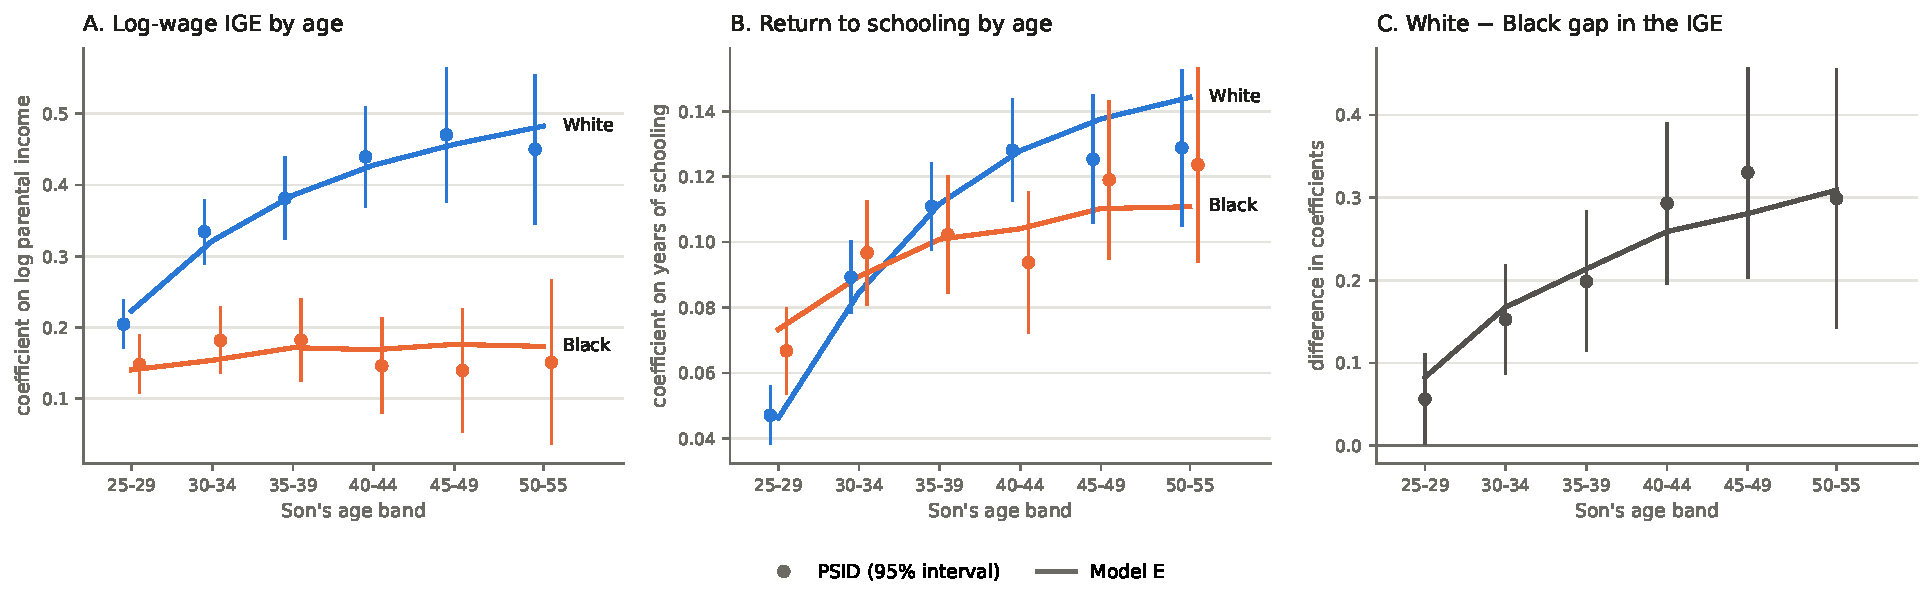
\includegraphics[width=\textwidth]{fig_model_fit.pdf}
\caption{Fit of the selected model (E): the log-wage IGE and the return to schooling by age and race, and the White
$-$ Black gap in the IGE}\label{fig:modelfit}
\par\smallskip
\begin{minipage}{\textwidth}\footnotesize \textit{Notes:} PSID sons, coefficients by five-year band with single-age
dummies, 95\% intervals from 500 cluster-bootstrap draws (the gap's from the same draws); model E at its estimates with
the PSID observation scheme, twenty simulated sons per PSID son. All 66 targeted moments with their $t$ ratios are in
Appendix Table~\ref{tab:modelfit}. Code: \texttt{model/figure\_fit.py}.\end{minipage}
\end{figure}

\paragraph{Fit.} The model reproduces the puzzle (Figure~\ref{fig:modelfit}; all moments in Appendix
Table~\ref{tab:modelfit}). The White IGE rises from 0.223 at 25--29
to 0.457 at 45--49 (PSID 0.205 and 0.470) and the Black IGE stays between 0.140 and 0.176 (PSID 0.140--0.182); the gap
is 0.168 at 30--34 and 0.281 at 45--49 (PSID 0.153 and 0.330). The
model also reproduces a moment it was not fitted to: the same-employer growth gradient in parental income at 25--34 is
0.018 (White) and 0.001 (Black) in the model, against 0.019$^{***}$ (s.e.\ 0.006, $p = 0.001$) and 0.007 (0.008) in the
PSID; net of schooling 0.008 and $-0.001$, against 0.006 (0.006) and 0.005 (0.009).\footnote{Untargeted. The statistic is computed on the model's stayer pairs (consecutive interviews one to two
years apart from 1985, same employer, no displacement, a wage at both, ages 25--34), without the age and year controls
of Table~\ref{tab:growthladder}, whose values on its own sample are 0.021$^{***}$ (0.006) for White and 0.003 (0.008)
for Black sons; the model is compared with the statistic computed the same way on the PSID. Code:
\texttt{model/core.py} (\texttt{untargeted}), PSID values with 300 cluster-bootstrap draws in
\texttt{model/output/untargeted\_psid.json}.}

\paragraph{Untargeted validation.} Table~\ref{tab:modeluntargeted} compares the model with statistics it was not fitted
to, computed with the same code on the PSID and on the simulated panel.

\begin{table}[!htbp]
\centering
\caption{Untargeted validation of the selected model (E)}
\label{tab:modeluntargeted}
\resizebox{\ifdim\width>\textwidth\textwidth\else\width\fi}{!}{%
\begin{tabular}{lcccc}
\toprule
Statistic & PSID & (s.e.) & Model & $t$ \\
\midrule
\multicolumn{5}{l}{\textit{Mean log wage}} \\
\quad White, 35--39 & $2.914$ & (0.019) & $3.022$ & $5.7$ \\
\quad Black, 35--39 & $2.489$ & (0.019) & $2.596$ & $5.5$ \\
\quad White, 45--49 & $3.032$ & (0.023) & $3.179$ & $6.5$ \\
\quad Black, 45--49 & $2.614$ & (0.028) & $2.708$ & $3.4$ \\
\quad White $-$ Black, 35--39 & $0.425$ & (0.027) & $0.426$ & $0.1$ \\
\quad White $-$ Black, 45--49 & $0.418$ & (0.036) & $0.472$ & $1.5$ \\
\multicolumn{5}{l}{\textit{Rank--rank slope (son's wage percentile on parental-income percentile)}} \\
\quad White, 25--29 & $0.251$ & (0.020) & $0.251$ & $-0.0$ \\
\quad White, 30--34 & $0.342$ & (0.022) & $0.331$ & $-0.5$ \\
\quad White, 45--49 & $0.379$ & (0.036) & $0.391$ & $0.3$ \\
\quad Black, 25--29 & $0.199$ & (0.028) & $0.187$ & $-0.4$ \\
\quad Black, 30--34 & $0.212$ & (0.029) & $0.188$ & $-0.8$ \\
\quad Black, 45--49 & $0.192$ & (0.053) & $0.178$ & $-0.3$ \\
\quad White $-$ Black, 25--29 & $0.052$ & (0.036) & $0.064$ & $0.3$ \\
\quad White $-$ Black, 45--49 & $0.187$ & (0.062) & $0.213$ & $0.4$ \\
\multicolumn{5}{l}{\textit{Share whose modal job at 35--55 is a $G$ job}} \\
\quad White, bottom parental tercile & $0.088$ & (0.018) & $0.030$ & $-3.2$ \\
\quad White, top parental tercile & $0.227$ & (0.015) & $0.131$ & $-6.6$ \\
\quad Black, bottom parental tercile & $0.044$ & (0.009) & $0.020$ & $-2.7$ \\
\quad Black, top parental tercile & $0.122$ & (0.033) & $0.073$ & $-1.5$ \\
\multicolumn{5}{l}{\textit{Log-wage IGE below the median of parental income}} \\
\quad White, 25--29 & $0.107$ & (0.053) & $0.258$ & $2.8$ \\
\quad White, 45--49 & $0.295$ & (0.153) & $0.419$ & $0.8$ \\
\quad Black, 25--29 & $0.130$ & (0.028) & $0.140$ & $0.4$ \\
\quad Black, 45--49 & $0.112$ & (0.052) & $0.162$ & $0.9$ \\
\multicolumn{5}{l}{\textit{Parental-income gradient of log wages without / with a $G$-job dummy}} \\
\quad White, 25--34, without & $0.258$ & (0.018) & $0.270$ & $0.7$ \\
\quad White, 25--34, with & $0.243$ & (0.018) & $0.257$ & $0.8$ \\
\quad White, 35--55, without & $0.421$ & (0.031) & $0.426$ & $0.2$ \\
\quad White, 35--55, with & $0.387$ & (0.031) & $0.406$ & $0.6$ \\
\quad Black, 25--34, without & $0.157$ & (0.020) & $0.155$ & $-0.1$ \\
\quad Black, 25--34, with & $0.146$ & (0.019) & $0.148$ & $0.1$ \\
\quad Black, 35--55, without & $0.158$ & (0.028) & $0.173$ & $0.5$ \\
\quad Black, 35--55, with & $0.141$ & (0.027) & $0.167$ & $0.9$ \\
\multicolumn{5}{l}{\textit{Same-employer growth at 25--34 on log parental income}} \\
\quad White & $0.019$ & (0.006) & $0.019$ & $-0.1$ \\
\quad Black & $0.007$ & (0.008) & $0.002$ & $-0.6$ \\
\quad White, net of schooling & $0.006$ & (0.006) & $0.009$ & $0.4$ \\
\quad Black, net of schooling & $0.005$ & (0.009) & $0.000$ & $-0.6$ \\
\bottomrule
\end{tabular}}
\par\smallskip
\begin{minipage}{\textwidth}\footnotesize \textit{Notes:} None of these statistics is a target. PSID: the sons' panel of the targets, 300 cluster-bootstrap draws of 1968 families. Model: model E at its estimates, mean over ten simulation seeds, 20 simulated sons per PSID son, the same code (\texttt{model/core.py}, \texttt{validation} and \texttt{untargeted}) on the simulated panel with the PSID observation scheme. $t$ = (model $-$ PSID) / PSID s.e. Ranks: percentile of the son's log wage among Black and White sons in the band and of parental income among the same sons. Output: \texttt{model/output/validation\_psid.json}, \texttt{final\_x4/validation\_E.json}; code \texttt{model/validation\_run.py}.\end{minipage}
\end{table}


\noindent Five statistics pass and three fail.
\begin{enumerate}[leftmargin=*, itemsep=0pt]
\item The racial wage gap widens with age as in the data: 0.426 at 35--39 and 0.472 at 45--49 in the model, 0.425
(0.027) and 0.418 (0.036) in the PSID; only the gap at 25--29 is targeted. The levels fail: the model's wages at 35--49
are 0.09--0.15 log points above the PSID for both races ($t$ between 3.4 and 6.5), with the level at 25--29 fitted;
the failure is wage growth within sons in their thirties that is too fast by 0.11, not the selection of who
has a wage (Appendix~\ref{app:modeldiag}).
\item Rank--rank slopes of sons' hourly wages on parental income match at every band and for both races ($|t| < 1$):
White 0.251, 0.331 and 0.391 at 25--29, 30--34 and 45--49 in the model against 0.251, 0.342 and 0.379, Black 0.187,
0.188 and 0.178 against 0.199, 0.212 and 0.192. On this sample and in hourly wages the PSID's rank slopes diverge by race, from
0.052 (0.036) at 25--29 to 0.187$^{***}$ (0.062, $p = 0.003$) at 45--49 (model 0.064 and 0.213), as own-earnings ranks do
at 40--44 (Table~\ref{tab:rankage}, 0.150$^{*}$); the ranks that do not
diverge in Section~\ref{sec:ageprofile} are ranks of family income.
\item The parental-income gradient of log wages of White sons at 35--55 falls by 0.034 (8\%) in the PSID and by
0.020 (5\%) in the model when a dummy for a $G$ job is added (0.421 to 0.387 and 0.426 to 0.406), and that of Black sons
by 0.011--0.016 in the PSID and 0.006--0.007 in the model: the job type carries a part of the gradient, accumulation
within job types the rest.
\item Below the median of parental income the Black IGE matches (0.140 and 0.162 at 25--29 and 45--49, against 0.130 and
0.112, $|t| \le 0.9$); the White IGE below the median is too high at 25--29 (0.258 against 0.107, $t = 2.8$) and rises
by about as much as in the PSID to 45--49 (0.16 against 0.19). The model is linear in parental income, and the data's
White gradient at the bottom is flatter at entry.
\item The share of sons whose modal job at 35--55 is a $G$ job fails: 0.131 against 0.227 for White sons from the top
tercile ($t = -6.6$), 0.030 against 0.088 from the bottom; for Black sons 0.073 against 0.122 and 0.020 against 0.044.
In the PSID the share in $G$ jobs rises with age for White sons and is stable for Black sons; in the model it falls
after 30--34, because the model loses $G$ jobs through moves and displacement, while in the PSID $G$ jobs are lost at
half the rate of $O$ jobs. A job-loss rate specific to good jobs is the next step (Appendix~\ref{app:modeldiag}).
\item The same-employer growth gradient in parental income passes (Fit, above).
\end{enumerate}

\subsection{Counterfactuals}

\begin{table}[!htbp]
\centering
\caption{Counterfactuals in the selected model (E)}
\label{tab:modelcf}
\resizebox{\ifdim\width>\textwidth\textwidth\else\width\fi}{!}{%
\begin{tabular}{lcccc}
\toprule
Experiment & IGE gap, 30--34 & IGE gap, 45--49 & Log wage 25--34, Black & Log wage 25--34, White \\
\midrule
Baseline: White $-$ Black gap & $0.168^{***}$ (0.031) & $0.281^{***}$ (0.044) & 2.397 & 2.718 \\
\midrule \multicolumn{5}{l}{\textit{Change from the baseline}} \\
Equal pay-off of parental income in accumulation (H4 off) & $-0.120^{***}$ (0.032) & $-0.166^{***}$ (0.045) & -0.046 & 0.000 \\
Equal pay-off of schooling in accumulation (H2 off) & $-0.025^{***}$ (0.009) & $-0.035^{***}$ (0.012) & 0.023 & 0.000 \\
Equalising schooling & $-0.013^{***}$ (0.002) & $-0.024^{***}$ (0.003) & 0.011 & 0.000 \\
Equal access to $G$ jobs by parental income ($\alpha_1 = 0$) & $-0.002$ (0.002) & $-0.005$ (0.004) & 0.000 & -0.001 \\
Equal displacement risk ($\delta_{0B} = \delta_{0W}$) & $0.006^{***}$ (0.002) & $0.007^{***}$ (0.003) & 0.033 & 0.000 \\
Equal job finding out of work ($\Delta\ell_u = 0$) & $0.004^{**}$ (0.002) & $0.005$ (0.003) & 0.015 & 0.000 \\
Recession at entry (+3 points for three years) & $-0.002^{*}$ (0.001) & $-0.003^{*}$ (0.001) & -0.021 & -0.012 \\
\bottomrule
\end{tabular}}
\par\smallskip
\begin{minipage}{\textwidth}\footnotesize \textit{Notes:} Simulated at the estimates of model E with the PSID sons' race, parental income, schooling and birth years and the PSID observation scheme, 20 simulated sons per PSID son. First row: baseline White $-$ Black gap in the log-wage IGE and mean log wages; other rows: changes from it. The racial wage level $\mu_B$ is held fixed. H4 off: Black sons get White sons' pay-off of parental income in accumulation; because Black sons' parental income is mostly below the pooled mean around which the term is centred, this raises the Black IGE and lowers the mean Black wage; it is a decomposition of the gap, not a policy. Equalising schooling: Black sons' schooling drawn from White sons' within the same parental-income decile. Recession at entry: national unemployment 3 points higher in each son's first three years in the labor market. Delta-method standard errors (same draws at every parameter value); $^{***}$ $p<0.01$, $^{**}$ $p<0.05$, $^{*}$ $p<0.1$. Code: \texttt{model/postestimation.py}; output \texttt{model/output/postestimation\_Lx4\_E.json}.\end{minipage}
\end{table}


Table~\ref{tab:modelcf} switches off each channel in the selected model, with the racial wage level held fixed. Giving
Black sons White sons' pay-off of parental income in accumulation closes 0.120$^{***}$ (s.e.\ 0.032) of the 0.168 gap at
30--34 and 0.166$^{***}$ (0.045) of the 0.281 gap at 45--49, both $p < 0.001$: seven tenths and three fifths. This is
a decomposition, not a policy: it closes the gap by making Black sons' wages depend on parental income as White sons'
do, which raises the Black IGE and, because most Black sons' parents are below the pooled mean of parental income, lowers
the mean Black wage at 25--34 by 0.046. Giving Black sons White sons' pay-off of schooling in accumulation closes
0.025$^{***}$ and 0.035$^{***}$ ($p = 0.005$ and 0.006) and raises the Black wage at 25--34 by 0.023. Equalising
schooling within parental-income deciles closes 0.013$^{***}$ at 30--34 and 0.024$^{***}$ at 45--49 ($p < 0.001$), 8\%
and 9\% of the gap. Equal access to good jobs across parental income changes nothing ($-0.005$, $p = 0.22$); equal
displacement risk widens the gap by 0.007$^{***}$ at 45--49 ($p = 0.008$), 3\% of it, while raising Black wages by
0.033; and a recession at entry narrows it by 0.003$^{*}$ ($p = 0.07$). Giving Black sons White sons' job finding out
of work raises Black wages at 25--34 by 0.015$^{***}$ (s.e.\ 0.003, $p < 0.001$), 5\% of the racial wage gap there,
and more for sons from the bottom tercile of parental income (0.038$^{***}$ at 45--49) than from the top
(0.030$^{***}$), so it widens the IGE gap by 0.004$^{**}$ at 30--34 ($p = 0.036$) and 0.005 at 45--49 ($p = 0.11$):
the search friction out of work is a channel of the racial wage level, not of persistence. \citet{rauh2023black} find
the same separation for the level of wages in a model where the employment gap comes from preferences: giving Black men
White men's preferences over work closes 44\% of the employment gap (0.149 to 0.083) and 7\% of the hourly-wage gap
(0.355 to 0.331).

\paragraph{Search frictions in two generations.} A search friction can hold back the father as well as the son. In the
son's generation it does not shape the profile. The share of zero-hours years falls with parental income at the same
rate for Black and White sons ($-0.027^{***}$ and $-0.022^{***}$, difference $-0.006$, s.e.\ 0.011, $p = 0.59$; at
equal schooling $p = 0.76$); imputing a wage to every zero-hours year, at the son's last wage or at the tenth
percentile of his race and age band, leaves the racial gap in the opening of the IGE between 25--29 and 45--49 at
0.255$^{***}$ and 0.283$^{***}$, against 0.274$^{***}$ on observed wages; and fixed effects for the state at 17 leave
it at 0.307$^{***}$ (0.313$^{***}$ without them, same sons). In the father's generation it carries part of the
opening. The father's shares of the son's childhood years displaced, unemployed and with zero hours account for 13\%
(White) and 16\% (Black) of the variance of parental income. Among sons with a resident father, measuring parental
income over the father's years without displacement, unemployment or zero hours leaves the racial gap in the opening
where it was (0.148 and 0.142, change $-0.006$, s.e.\ 0.016, $p = 0.69$): the father's spells do not distort parental
income as a measure. The father's instability itself matters for young Black sons: holding the three shares fixed
lowers the Black IGE at 25--29 by 0.028$^{**}$ (s.e.\ 0.012, $p = 0.024$) and the racial gap in the opening by
0.061$^{*}$ ($p = 0.094$), from 0.204$^{**}$ to 0.143, three tenths of it. Part of young Black sons' wage persistence
runs through their fathers' instability, which flattens the Black profile. The model takes parental income as data and
has no family-level instability, so this part sits inside its pay-off of parental income in accumulation. Search
friction does pass from father to son: a son whose father had a year displaced, unemployed or with zero hours in the
window is 0.131$^{***}$ (White) and 0.123$^{***}$ (Black) more likely to be in the third of sons with the most such
years over the career ($p < 0.001$). The part of the IGE that runs through both generations' employment---the son's
inherited friction times what it costs him---is 0.005$^{***}$ ($p = 0.005$) of the White wage IGE at 25--29, 2\% of it,
and 0.005 ($p = 0.21$), 3\%, of the Black; in annual earnings 0.010$^{***}$ and 0.015 ($p = 0.21$), 5\% and 6\%. It
does not grow with age (0.000 and $-0.009$ from 25--29 to 45--49) and carries 5\% of the racial gap in the opening
(0.010, s.e.\ 0.011, $p = 0.38$).\footnote{Exact decomposition of the IGE into the paths through the father's and the
son's friction (shares of years displaced, unemployed or with zero hours), sons with a resident father, 200
cluster-bootstrap draws of 1968 families. Leaving out the pairs in which both generations had such years lowers the
White wage IGE by 0.032$^{***}$ to 0.066$^{***}$ across bands and the Black earnings IGE by 0.076$^{**}$ to
0.140$^{**}$, equally by race in the opening ($-0.014$, s.e.\ 0.049): these pairs carry the level of persistence, not
its racial rise. Code: \texttt{IGE/73.SharedFriction.py}; output \texttt{output/shared\_friction.md}.} The racial
difference in that pay-off is not a matter of how Black fathers' income is measured: with the father's years of
schooling, fixed before he meets the labor market, as the background measure, a year of it adds 0.021$^{***}$ (s.e.\
0.006, $p < 0.001$) to White sons' ten-year wage growth at equal own schooling and 0.000 to Black sons', a difference of
0.021$^{*}$ ($p = 0.051$), and 0.025$^{**}$ ($p = 0.033$) with parental income held fixed.\footnote{Sons 25--55,
log-wage IGE by five-year band with single-age dummies, s.e.\ clustered by 1968 family; the changes in the opening are
from 200 cluster-bootstrap draws of families. Father's shares and clean-year income over the son's childhood window
(Section~\ref{sec:fathers}; \texttt{IGE/24.IGEDecomposition.py}); state at 17 from the family file, 1976 onward. In levels the father's
schooling coefficient rises with age for both races (0.046$^{***}$ White, 0.033$^{***}$ Black, from 25--29 to 45--49);
the racial difference is in the growth of the same sons' wages. Code: \texttt{IGE/72.FrictionGenerations.py}; output
\texttt{output/friction\_generations.md} and \texttt{friction\_generations\_boot.json}.}


\paragraph{Which sons, which ages.} Appendix Table~\ref{tab:modelcfh4} shows where the H4 decomposition acts. It raises the Black
IGE by 0.087$^{***}$ (0.024) at 25--29 and by 0.173$^{***}$ (0.047) at 50--55, so the part of the gap it carries grows
with every band. It carries a level as well as an opening: at 25--29 the model's gap is 0.083 and switching H4 off closes
0.087 of it, so of the opening between 25--29 and 45--49 (0.198 in the model) H4 carries 0.079, two fifths; the pay-off
of schooling and the race-neutral channels---schooling, access to $G$ jobs and job loss, which raise the White IGE more
than the Black---carry the rest. At 45--49 it raises the wage of Black sons from the top tercile of parental income by 0.088$^{***}$
(0.024) and lowers that of sons from the bottom tercile by 0.140$^{***}$ (0.038), both $p < 0.01$: the sons the racial
difference holds back are the sons of richer Black parents, whose wages do not grow with their parents' income as White
sons' do. Switching the pay-off of parental income off for both races shows how much of the White profile it builds: it
lowers the White IGE by 0.067$^{***}$ (0.025) at 25--29 and by 0.155$^{***}$ (0.058, $p = 0.008$) at 45--49, 34\% of its
level at 45--49 and 37\% of its rise from 25--29 in the model (0.087 of 0.234); the rest of the White rise comes through
schooling, access to $G$ jobs and job loss, which act for both races.

The counterfactuals answer the policy question the paper started from. Equalising the starting point---schooling,
access, entry conditions---closes less than a tenth of the gap at 45, because the gap is built by what parental income
and schooling buy in growth over the career. In the model a policy scored at 30 sees 60\% of the gap at 45; in the PSID it sees 46\% (0.153 of 0.330),
because the model's gap at 30--34 is above the PSID's (0.168 against 0.153) and its gap at 45--49 below (0.281
against 0.330; Table~\ref{tab:modelfit}).

\paragraph{What policy could reach the channel.} The channel that carries the gap is the growth of a son's wage with
his parents' income at equal schooling and job type, for White sons and not for Black sons. The policies the model can
score---schooling, access to good jobs, entry conditions, job loss---act on where careers start and on their
interruptions, and none of them reaches it. What it consists of, public data observe only in part, and only in the
NLSY79, where the growth gradient at equal schooling is itself not significant (0.007, s.e.\ 0.006, for White sons at
25--34). There, the items that rise with parental income do not carry it: company training (0.020$^{***}$, s.e.\
0.006) and the size of the employer (0.387$^{***}$ log points, s.e.\ 0.098) rise with parental income for White sons,
union coverage does not (0.021, s.e.\ 0.015), and holding training, union coverage, employer size and tenure fixed
leaves the gradient unchanged (0.007; explained 0.000, s.e.\ 0.001); a job found through friends or relatives grows
more slowly ($-0.014^{***}$, s.e.\ 0.004) and accounts for 0.001$^{**}$ of the gradient; and in the PSID, following the
father's industry raises the starting wage, not its growth.\footnote{Code: \texttt{IGE/36.SameEmployerGrowthChecks.py}
(Section C, NLSY79 same-employer pairs) and \texttt{IGE/32.IndustryCareers.py} (following the father's industry,
PSID).} A policy aimed at the channel would have to act on what happens to equally schooled men inside their jobs over
the first twenty years of the career; the public data name the channel and bound it, but do not observe the employer.

\subsection{What the model leaves open}\label{sec:modelopen}

The model fits the age profile of persistence but not every career moment. The largest remaining misfits are the autocovariance
($-3.6$) and variance ($-3.3$) of stayers' wage growth, the wage gain at a move for Black sons ($+3.5$) and the variance
of Black log wages at 45--49 ($+3.5$), which falls in the data between 35--39 and 45--49 (0.382 to 0.345). The fall is not attrition on
observables: reweighting the moments for being observed, on parental income, income at 25--29, sample and cohort,
leaves the Black variance at 45--49 at 0.346 and moves the White $-$ Black opening of the IGE from 0.274 to 0.267, so the
attrition-weighted moment set changes none of the facts the race parameters are identified from.\footnote{The weights
are those of the attrition analysis of Section~\ref{sec:ageprofile} (inverse predicted probability of being observed in
each band, clipped at 20) on the 4,162 sons with family income at 25--29. Largest changes in target standard errors: the
Black IGE at 35--44 ($+0.9$) and the Black share of zero-hours years ($+1.4$). At the lattice's estimates of model E the criterion
on the weighted set is 113.7, with 3.6 from the IGE moments; its re-estimation on that set is the robustness
estimate. Code: \texttt{model/ipw\_build.py}, \texttt{ipw\_moments.py}; output
\texttt{model/output/ipw\_moments.md}, \texttt{data\_moments\_ipw.json}.} The
model also under-predicts the wage scar of entering in a recession ($-0.007$ and $-0.004$ a point, Black and White,
against $-0.013^{**}$ in Section~\ref{sec:policy}). Of the untargeted statistics, the model misses the level of wages after 35 (0.09--0.15 too high,
both races, through growth within sons), the share in good jobs after 35 (too low by 0.05--0.09, through moves and
displacement) and the White IGE below the median of parental income at 25--29 (0.26 against 0.11). The racial difference in job finding out of work fits non-employment by race and leaves the gain at a move where it
was. In the PSID the gain at a move falls with parental income for Black sons and not for White sons ($-0.069^{**}$,
$p = 0.015$, at 25--34; $-0.059^{**}$, $p = 0.025$, at 35--55), and the difference sits in the wage of the new job
(at 35--55 and equal schooling $-0.175^{**}$, $p = 0.016$, against $-0.068$, $p = 0.33$, for the old one), after short
tenure and in $O$ jobs; the PSID's one-year parental measure keeps it at 25--34 ($-0.050^{**}$, $p = 0.032$). The
NLSY79, with five times as many Black movers, does not show it (0.006, s.e.\ 0.013, at 25--34; $-0.002$ at 35--55;
also at equal schooling and AFQT), so the data sets differ, not the measures; the model does not target
it.\footnote{Consecutive interviews one to two years apart with a wage at both; PSID moves exclude displacement,
NLSY79 moves are employer changes between rounds. Code: \texttt{IGE/71.MoveGainAnatomy.py}; output
\texttt{output/move\_gain\_anatomy.md}.} The share in good jobs after 35 asks for a
lower job-loss rate in $G$ jobs, not for access that rises with age; the step is coded with the four shares at 35--55 as
added targets, and its estimation is the next one.

\subsection{A prediction for administrative data}

The PSID fact can be checked in administrative data when the cohorts measured by \citet{chetty2020race}, born 1978--83,
reach their mid-forties between 2023 and 2028. If the profile documented here holds, the White--Black gap in the log
elasticity of individual earnings measured at 43--47 should be 0.25--0.30, against about 0.10 at 31--37 for the same
cohorts, while rank--rank slopes of family income should change by less.
